\documentclass[UTF8,12pt]{article}
\usepackage{ctex}      %中文
\usepackage{graphicx}  %图片
\usepackage{geometry}  %页面间距
\usepackage{lastpage}
\usepackage[final]{pdfpages}%封面
\usepackage{listings}  %插入代码
\usepackage{color}
\usepackage{xcolor}
\usepackage{booktabs}  %table
\usepackage{float}

\definecolor{dkgreen}{rgb}{0,0.6,0}
\definecolor{gray}{rgb}{0.5,0.5,0.5}
\definecolor{mauve}{rgb}{0.58,0,0.82}

\lstset{%代码风格
    frame=tb,
	language=Python,
	aboveskip=3mm,
	belowskip=3mm,
	showstringspaces=false,
	columns=flexible,
	basicstyle={\small\ttfamily},
	numbers=none,
	numberstyle=\tiny\color{gray},
	keywordstyle=\color{blue},
	commentstyle=\color{dkgreen},
	stringstyle=\color{mauve},
	breaklines=true,
	breakatwhitespace=true,
	tabsize=3
}

\geometry{left=3cm,right=3cm,top=2.5cm,bottom=3.5cm}

\begin{document}
	
	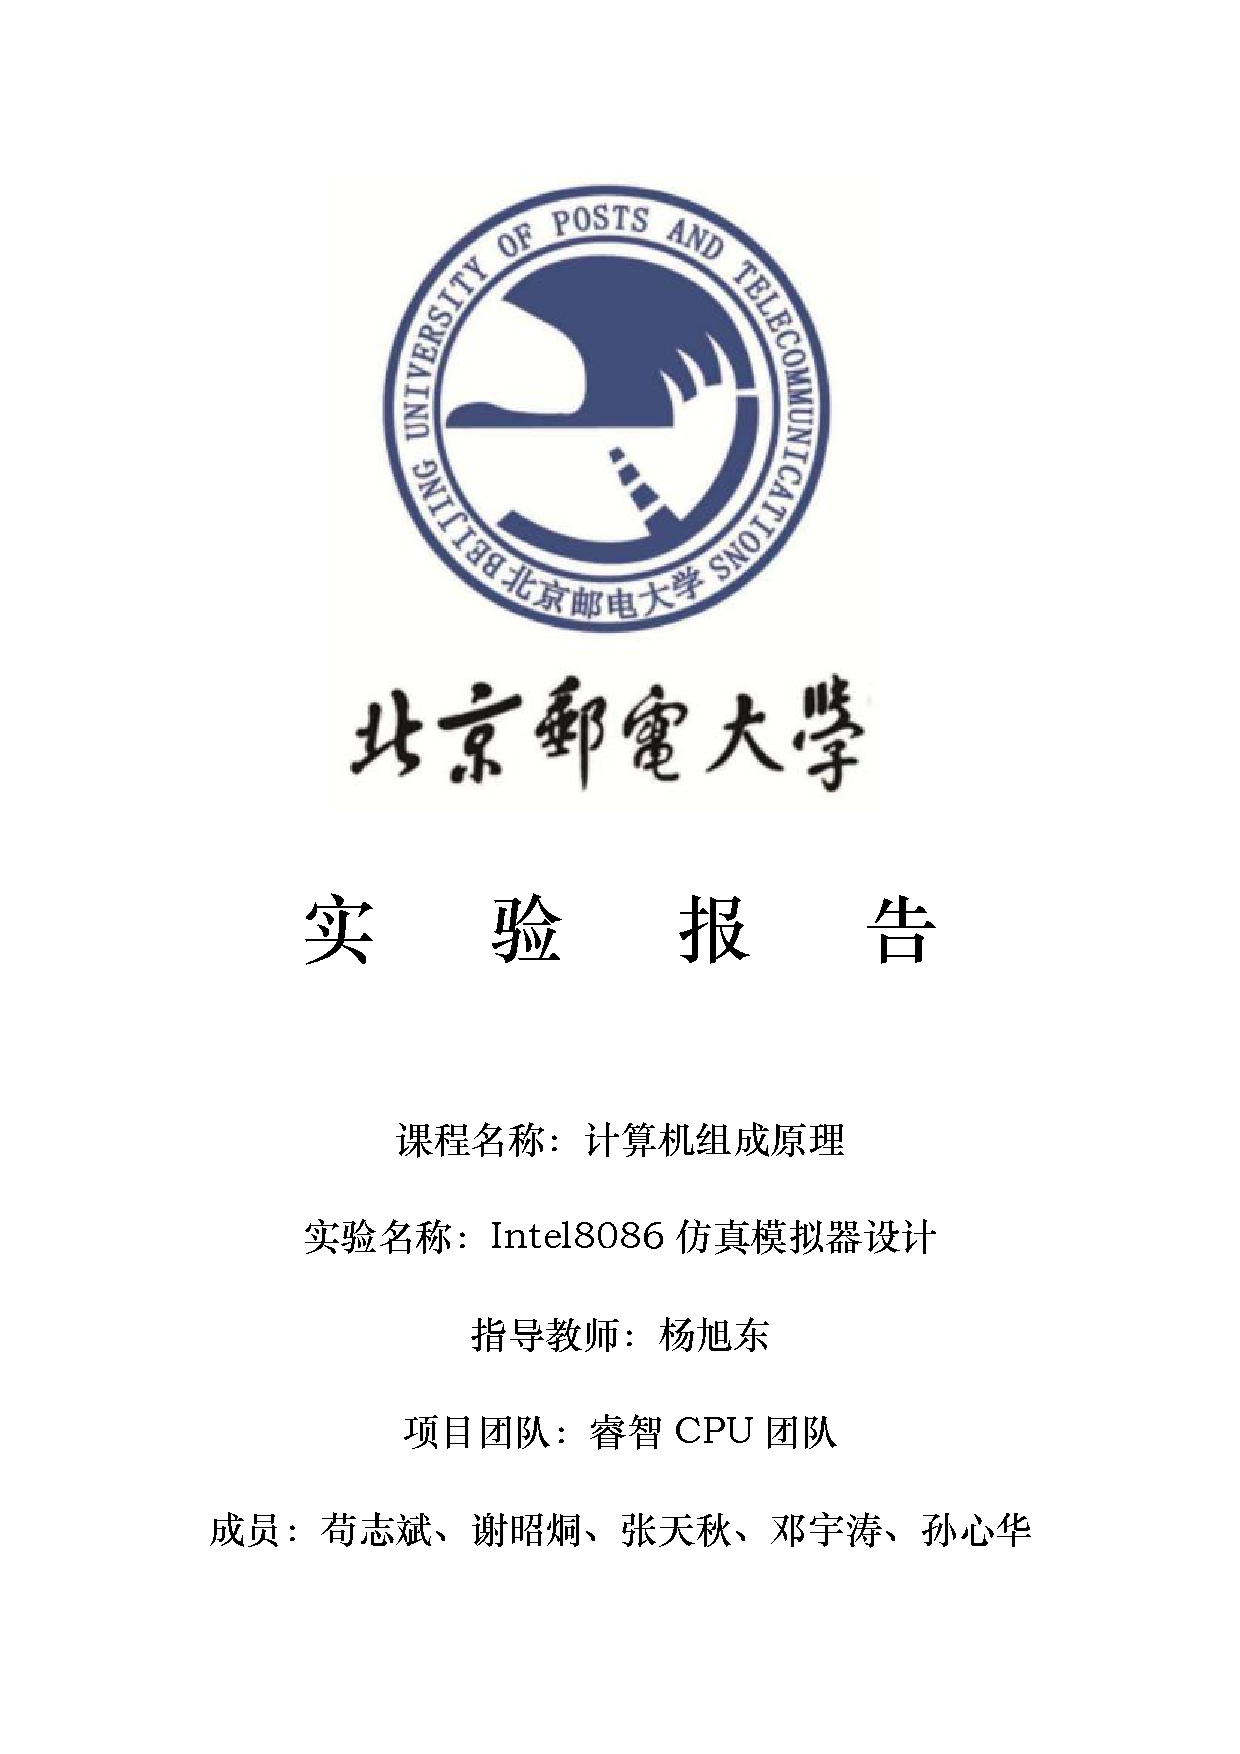
\includepdf{cover.pdf} %封面
	
	\tableofcontents
	\newpage
	%---------------------------------------------------------------------------------------%
	\section{实验目的}	
	通过团队合作,设计仿真模拟器,深入了解计算机内部寄存器、总线、I/O接口等工作原理,巩固计算机组成原理中学到的的操作数寻址方式等内容。
	
	%---------------------------------------------------------------------------------------%
	\section{运行环境}
	在Windows10环境下,基于python3.8集成开发环境,模拟实现Intel8086仿真模拟器。
	
	%---------------------------------------------------------------------------------------%
	\section{实验设计}
	在仿真模拟器设计实验中,我们队选择了Intel
	8086仿真模拟器进行设计。在我们的设计中,设置8086(x86构架的开端)所有的内部寄存器、内部及外部数据总线都是16位宽,是完全的16位微处理器,采用小端模式。20位外部地址总线,物理定址空间为1MB。
	%-----------------------%
	\subsection{总流程设计}
	
	\begin{figure}[!htb]
		\centering
		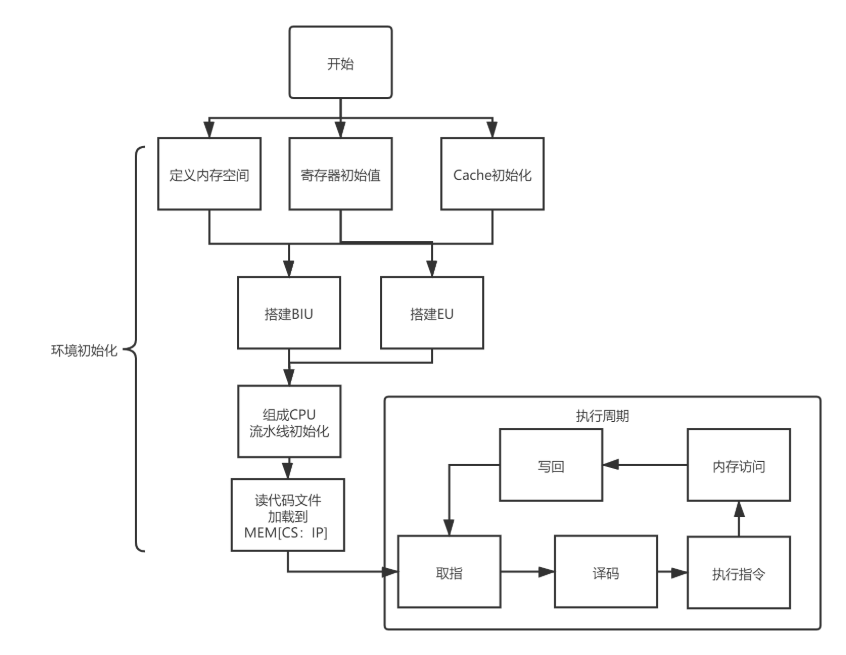
\includegraphics[width=10cm]{fig/flow-chart}
	\end{figure}
	
	
	%-----------------------%
	\subsection{模块功能划分及参数设定}
	
	\begin{itemize}
		\item \textbf{主函数:main.py}
		
		\begin{lstlisting}		
		MEMORY_SIZE = int('FFFFF', 16)   # 内存空间大小
		DATA_SEGMENT = int('20000', 16)  # 数据段
		CODE_SEGMENT = int('30000', 16)  # 代码段
		STACK_SEGMENT = int('50000', 16) # 栈段
		EXTRA_SEGMENT = int('70000', 16) # 其他段
		SEGMENT_SIZE = int('10000', 16)  # 段长度均为最大长度64kB(10000H)
		CACHE_SIZE = int('10000', 16)    # 缓存大小
		INSTRUCTION_QUEUE_SIZE = 6     	 #指令长度
		\end{lstlisting}
		
		\item \textbf{CPU运算:cpu.py}
		
		模拟CPU运算时过程,将一个CPU周期划分取指周期和执行周期,并打印运行时状态。
		
		\begin{lstlisting}
		class CPU(object) #将CPU定义为类,方便调用
		\end{lstlisting}
		
		\item \textbf{内存存储数据:memory.py}
		
		模拟内存存储,包含内存初始化、内存溢出、读写以字或字节为单位的数据(小端方式)以及cache高速缓存处理方式。
		
		\begin{lstlisting}
		class Memory(object) #将内存存储定义为类,方便调用		
		\end{lstlisting}
		
		\item \textbf{寄存器存储:register.py}
		
		对数据寄存器:AX、BX、CX、DX,指针寄存器:SP、BP,变址寄存器:SI、DI,控制寄存器:IP、FLAG,段寄存器:CS(代码段)、DS(数据段)、SS(堆栈段)、ES(附加段)进行模拟。
		
		\begin{lstlisting}
		class General_register(object) #将通用寄存器定义为类,方便调用
		class Register(int) #将寄存器定义为类,方便调用
		class Flag_register(object) #将标志寄存器定义为类,方便调用
		class Register_file(object) #将寄存器堆定义为类,方便调用
		\end{lstlisting}
		
		\item \textbf{汇编处理器:assembler.py}
		
		汇编器对输入的汇编指令进行拆分,把字符类型的指令和数据都转化成数据存入相应的位置,再进行编译。
		
		\begin{lstlisting}
		data_def_ins = ['DB', 'DW', 'DD', 'DQ', 'DT', 'DUP'] #定义字形数据	
		class Assembler(object)	#将汇编器汇编过程定义为类,方便调用
		\end{lstlisting}
		
		\item \textbf{指令集:instruction.py}
		
		将指令集进行分类,分别存放在相应的list中。
		
		\begin{lstlisting}
		data_transfer_ins = ['MOV', 'XCHG', 'LEA', 'LDS', 'LES'] #数据传送指令
		arithmetic_ins = ['ADD', 'SUB', 'INC', 'DEC', 'MUL', 'IMUL', 'DIV', 'IDIV', 'INC', 'DEC', 'CBW', 'CWD'] #算术指令
		logical_ins = ['AND', 'OR', 'XOR', 'NOT', 'NEG', 'CMP', 'TEST'] #逻辑指令
		rotate_shift_ins = ['RCL', 'RCR', 'ROL', 'ROR', 'SAL', 'SHL', 'SAR', 'SHR'] #循环和移位指令
		transfer_control_ins = ['JMP', 'JA', 'JAE', 'JB', 'JBE', 'JC', 'JCE', 'JCXZ', 'JE', 'JG', 'JGE' 'JL', 'JLE', 'JNA', 'JNAE', 'JNB', 'JNBE', 'JNC', 'JNE', 'JNG', 'JNE', 'JNG', 'JNGE', 'JNL', 'JNLE', 'JNO', 'JNP', 'JNS', 'JNZ', 'JO', 'JP', 'JPE', 'JPO', 'JS', 'JZ', 'LOOP', 'LOOPE', 'LOOPNE', 'LOOPNZ', 'LOOPZ', 'RET', 'CALL', 'RET', 'RETF'] #转移指令
		string_manipulation_ins = ['MOVS', 'CMPS', 'LODS', 'STOS', 'SCAS', 'REP', 'REPE', 'REPZ', 'REPNE', 'REPNZ'] #字符串处理指令
		flag_manipulation_ins = ['STC', 'CLC', 'CMC', 'STD', 'CLD', 'STI', 'CLI', 'LANF', 'SANF'] #标志操作指令
		stack_related_ins = ['PUSH', 'POP', 'PUSHF', 'POPF'] #栈相关指令
		input_output_ins = ['IN', 'OUT'] #输入输出指令
		miscellaneous_ins = ['NOP', 'INT', 'IRET', 'XLAT', 'HLT', 'ESC', 'INTO', 'LOCK', 'WAIT'] #杂项说明指令
		
		\end{lstlisting}
		
		
		\item \textbf{总线接口单元:bus\_ineterface\_unit.py}
		
		从存储器中获取指令,从端口和存储器中读取数据,并将数据写入端口和高速存储器cache中。
		
		\begin{lstlisting}
		class bus_interface_unit(object) #将总线接口处理数据过程定义为类,方便调用
		
		\end{lstlisting}
		
		
		\item \textbf{执行单元:execution\_unit.py}
		
		对数据进行处理,实现数制转换,匹配指令并调用对应过程进行执行
		\begin{lstlisting}
		class execution_unit(object) #将指令执行过程定义为类,方便调用		
		\end{lstlisting}
		
	\end{itemize}
	

	%---------------------------------------------------------------------------------------%
	\section{测试说明}	
	    本次实验的测试用例采用8086汇编语言编写,伪指令包含MASM5.0核心指令,采用Small存储模型。我们首先设计出斐波那契数列汇编程序和冒泡排序汇编程序两个基本测试用例,并在此基础上设计了数据传送类、测试指令类、算术类、字符串类、综合类、查找类、基本要求测试用例类等汇编程序。
	    \subsection{测试程序集说明}
	    \begin{itemize}
	        \item \textbf{数据传送类} \\ \\
    	        \begin{tabular}{c|l}
    	            \hline
        	        程序名 & 程序功能 \\
        	        \hline
        	        address\_mode & 测试各种数据传送中的寻址模式 \\
        	        \hline
        	        jmp & 测试jmp类指令的测试程序 \\
        	        \hline
        	        lea & 测试lea类指令的测试程序 \\
        	        \hline
    	        \end{tabular}
	        
	        \item \textbf{测试指令类} \\ \\
	            \begin{tabular}{c|c|l}
	                \hline
	                程序名 & 类型 & 程序功能 \\
	                \hline
	                logical & 逻辑运算指令 & 测试各类逻辑运算指令的测试程序 \\
	                \hline
	                rotate\_and\_shift & 移位运算指令 & 测试各类移位运算指令的测试程序 \\
	                \hline
	                stack & 栈指令 & 测试栈指令的测试程序 \\
	                \hline
	                inout & 输入输出指令 & 测试输入输出指令的测试程序 \\ \hline
	            \end{tabular}
	            
	        \item \textbf{算术指令类} \\ \\
	            \begin{tabular}{c|l}
	                \hline
        	        程序名 & 程序功能 \\
        	        \hline
        	        add\_8b\_16b & 2个一字节数和2个二字节数的加法 \\ \hline
        	        add\_16b\_carry & 2个一字长数带进位的加法 \\ \hline
        	        add\_in\_memory & 完成连续地址单元中数的连续加法 \\ \hline
        	        divide\_16b\_by\_8b & 完成16bits数除以8bit的除法 \\ \hline
        	        multiply\_2\_32b & 两个32bits数的乘法 \\ \hline
        	        sub\_8b & 两个8bits数的减法 \\ \hline
        	        Sum\_of\_n\_8b & 数据段中连续空间中8bits数的和 \\ \hline
    	        \end{tabular}
    	        
    	    \item \textbf{字符串类} \\ \\
	            \begin{tabular}{c|l}
	                \hline
        	        程序名 & 程序功能 \\
        	        \hline
        	        copy\_string\_instruction & 将连续内存位置的字符串从一个内存复制到另一个内存 \\ \hline
        	        display\_characters & 输出一个字符 \\ \hline
        	        display\_string & 输出一个字串符 \\ \hline
        	        display\_time & 输出当前的时间 \\ \hline
        	        hello\_world\_string & 输出字符串"hello,world!" \\ \hline 
    	        \end{tabular}
    	        
    	   \item \textbf{查找类} \\ \\
	            \begin{tabular}{c|l}
	                \hline
        	        程序名 & 程序功能 \\
        	        \hline
        	        binary\_search & 二分查找的汇编程序 \\ \hline
    	        \end{tabular}
    	        
    	   \item \textbf{基本要求测试用例类} \\ \\
	            \begin{tabular}{c|l}
	                \hline
        	        程序名 & 程序功能 \\
        	        \hline
        	        fibonacci & 实现斐波那契数列的汇编程序 \\ \hline
        	        bubble\_sort & 实现冒泡排序的汇编程序 \\ \hline
    	        \end{tabular}
    	        
    	   \item \textbf{综合类} \\ \\
	            \begin{tabular}{c|l}
	                \hline
        	        程序名 & 程序功能 \\
        	        \hline
        	        average\_sum\_array & 求出一个数组中数据的平均值 \\ \hline
        	        count\_1 & 求出二进制中1的个数的汇编程序 \\ \hline
        	        fact & 求出一个正整数的阶乘的汇编程序 \\ \hline
        	        finding\_largest\_number\_memory & 从顺序存储在内存位置2000:5000H中的16个8位\\&数字的无序数组中找到最大的数字 \\ \hline
        	        gcd\_two & 求出两个数的最大公约数的汇编程序 \\ \hline
        	        given\_number\_prime & 判断给出的数是否为素数的汇编程序 \\ \hline
        	        power & 给出两个正整数a、b,求出$a^b$的汇编程序 \\ \hline
        	        reverse\_array & 求出给出数组的逆序的汇编程序 \\ \hline
        	        sum\_average\_unsigned & 求出一组无符号数之和与平均值 \\ \hline
    	        \end{tabular}
	    
	    \end{itemize}
	    \subsection{运行说明}
	    
	    \subsubsection{命令行界面运行说明}
	    示例汇编代码见tests文件夹,也可根据伪指令文档自行编写程序,运行如下:
	    \begin{lstlisting}
	    $ python main.py tests/Requirement/bubble_sort.asm
	    \end{lstlisting}
	    
	    \subsubsection{图形界面运行说明}
	    提供Windows环境下的.exe可执行程序与MacOS环境下的.app可执行程序,双击打开运行即可。
	    图形界面简介如下图:\\
	    \begin{figure}[H]
    	    \centering
    	    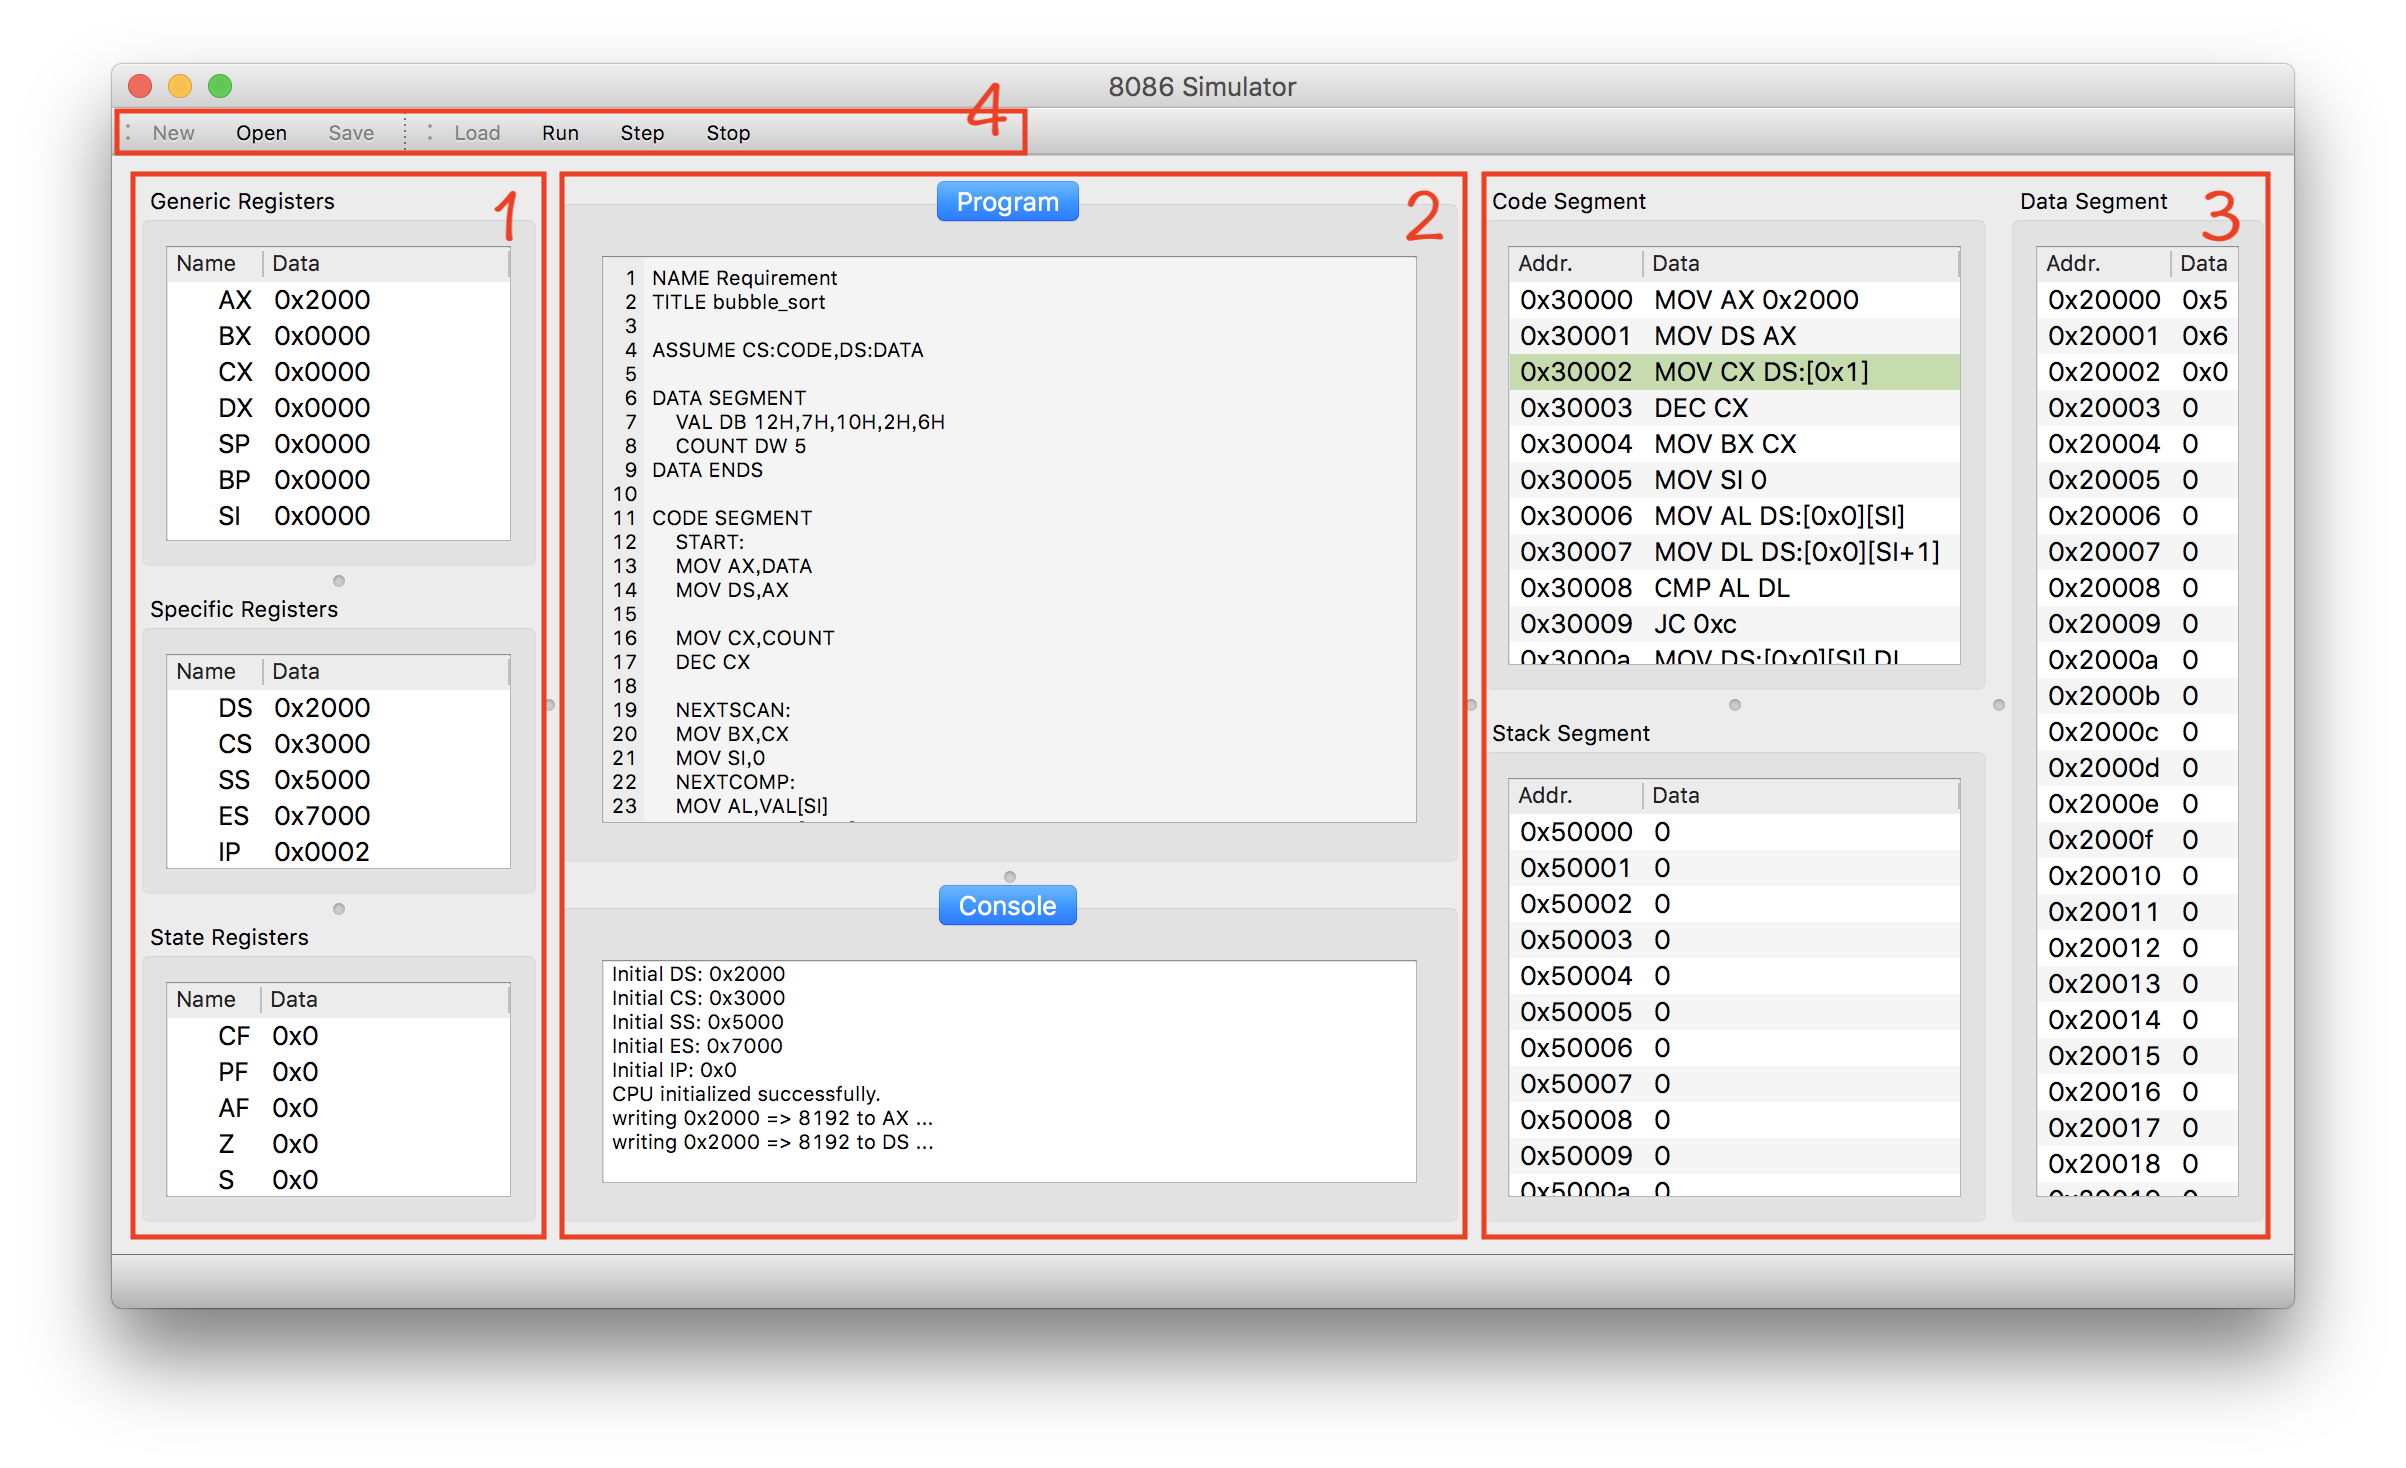
\includegraphics[width=15cm]{fig/ui.png}
    	    \caption{图形界面简介}
    	    \label{图形界面简介}
	    \end{figure}
	    区域1显示各寄存器所存储的值,包括通用寄存器部分、特殊寄存器部分和标识寄存器部分。
	    
	    区域2上半部分“Program”用于显示将被载入执行的汇编代码,该部分支持导入外部汇编代码文件和直接输入。汇编代码执行过程中的一些反馈信息于区域2下半部分“Console”中输出。
	    
	    区域3中三个部分分别显示指令部分、栈部分和数据部分对应的存储单元,当前待执行指令在指令部分的存储单元中提供高亮显示。
	    
	    区域4为菜单栏,其中“Open”为导入外部汇编代码文件;“Load”为载入当前“Program”部分的汇编代码;“Run”为连续执行,直至程序自然停止或者人为终止;“Step”为单步执行,即仅执行一个CPU周期;“Stop”为立即停止执行。
	    
	    
	    \subsection{基本要求汇编程序代码}
	    \begin{itemize}
	    \item \textbf{斐波那契数列汇编程序代码}
	    \begin{lstlisting}[language={[x86masm]Assembler}]
;Code for Program to Print the Fibonacci series in Assembly Language
NAME Requirement
TITLE fibonacci

ASSUME CS:CODE,DS:DATA

;Declaration Part
DATA SEGMENT
        RES DB ?
        CNT DB 18H       ; Initialize the counter for the no of Fibonacci No needed
DATA ENDS

CODE SEGMENT
        START: MOV AX,DATA
               MOV DS,AX
               LEA SI,RES
               MOV CL,CNT       ; Load the count value for CL for looping
               MOV AX,00H       ; Default No
               MOV BX,01H       ; Default No

               ;Fibonacci Part
               L1:ADD AX,BX
               MOV [SI],AX
               MOV AX,BX
               MOV BX,[SI]
               OUT 20h,AX 
               INC SI
               LOOP L1

               INT 3H           ; Terminate the Program
CODE ENDS
END START


	    \end{lstlisting}
	    
	    \item \textbf{冒泡排序汇编程序代码}
	    \begin{lstlisting}[language={[x86masm]Assembler}]
;ALP to Sort a set of unsigned integer numbers in ascending/ descending
;order using Bubble sort algorithm.
NAME Requirement
TITLE bubble_sort

ASSUME CS:CODE,DS:DATA

DATA SEGMENT
    VAL DB 12H,7H,10H,2H,6H
    COUNT DW 5
DATA ENDS

CODE SEGMENT 
    START:
    MOV AX,DATA
    MOV DS,AX 
    
    MOV CX,COUNT       
    DEC CX
       
    NEXTSCAN:
    MOV BX,CX
    MOV SI,0
    NEXTCOMP:
    MOV AL,VAL[SI]
    MOV DL,VAL[SI+1]
    CMP AL,DL
    JC NOSWAP
    MOV VAL[SI],DL
    MOV VAL[SI+1],AL
    NOSWAP:
    INC SI
    DEC BX
    JNZ NEXTCOMP
    LOOP NEXTSCAN
    
    
    print:
	        mov cx,count
	        xor si,si
    print_again:
		    mov al,VAL[si]
			out 0,al
			inc si
            CMP cx,si
			jg print_again
        

    MOV AH,4CH
    INT 21H
CODE ENDS
END START 

	    \end{lstlisting}
	    \end{itemize}
    	
	\subsection{实际运行截图}
	\begin{itemize}
	    \item \textbf{斐波那契数列运行结果}
	    \begin{figure}[H]
    	    \centering
%    	    \includegraphics{}
    	    \caption{斐波那契数列命令行运行结果}
    	    \label{斐波那契数列命令行运行结果}
	    \end{figure}


        \item \textbf{冒泡排序运行结果}
	    \begin{figure}[H]
    	    \centering
%    	    \includegraphics{}
    	    \caption{冒泡排序命令行运行结果}
    	    \label{冒泡排序命令行运行结果}
	    \end{figure} 
	 \end{itemize}
	%---------------------------------------------------------------------------------------%
	\section{实现过程遇到及解决的问题}
	1. 最初准备将寄存器也封装成一个类,采取继承和组合的方式均效果不佳,最后选择使用数字数据类型及字典表示每一个寄存器。
	
	2. 最初许多细节没有搞清楚急于实现,读了《汇编语言》(王爽著)后有了新的理解,重新构建了代码。
	
	3. python 的列表并不像 C/C++ 的数组对其内的元素限制类型,实现时把内存抽象成一个列表,在访问内存里的内容时,一位不熟悉python的组员以为需要返回 [列表元素],但列表内支持存放任意类型的数据,包括列表。
	
	4. 8086汇编程序的伪指令有较多的版本,为了简化汇编器的处理工作,采用MASM5.0的核心指令,并人为舍弃一些宏指令,最终通过汇编器(实际上是解释器)来对输入的8086汇编程序进行读入处理。
	
	%---------------------------------------------------------------------------------------%
	\section{小组成员及分工}	

    \begin{table}[H]
    \begin{tabular}{l|c}
    \hline
    成员  & 分工                                          \\ \hline
    苟志斌 & 搭建项目整体框架,MASM伪指令实现,汇编器,流水线                  \\ \hline
    谢昭烔 & 指令集具体实现,调试与测试代码,整理文档                        \\ \hline
    邓宇涛 & 整理8086指令集,实现图形界面与人机交互,文档编写                  \\ \hline
    张天秋 & 研究8086汇编语言,熟悉伪指令的功能和编写,寻找、设计8086汇编\\&程序用例,文档整理 \\ \hline
    孙心华 & 流程图设计,参与编写部分指令,文档编写                       \\ \hline
    \end{tabular}
    \end{table}
	
	%---------------------------------------------------------------------------------------%
	\section{合作感悟及个人体会}	
	\subsection{合作感悟}
	通过这次团队设计CPU模拟仿真器,我们体会到团体合作的重要性,一个人的力量很小,但是一群人的力量很大。我们深感在线合作平台的便捷,对GitHub、Overleaf、Process On等有了深入了解和应用。
	\subsection{个人体会}
	\begin{itemize}
	    \item 苟志斌:在本次项目中,我仔细研读了王爽《汇编语言》一书,查阅相关资料和手册,对8086汇编有较为深入的学习,并实现了一个汇编解释器;通过研究Intel开发手册及相关资料,参与模拟了CPU的运行过程,主要负责了内存、存储器和流水线等的实现,在实践中对CPU的运行机理有了更多的理解和把握,可谓是受益匪浅。我们团队协作,能够高度仿真地模拟8086,并运行MASM5.0标准的大多数汇编代码,是一件极富有成就感的事情!
	    \item 谢昭烔:在本次项目中,为了能够具体实现指令集,我阅读了《汇编语言》及相关文档手册,对于具体指令的实现机制及算法有了深入了解。同时也重新阅读了《深入理解计算机系统》一书的部分章节,将上学期学习的知识进行了温习。学习到8086汇编相关知识的同时也练习了python程序的编写。这是本人第一次与他人组队实现一个大作业/项目,感觉到团队力量的强大,由衷感谢四位队友!
	    \item 邓宇涛:在本次项目中,我前期阅读了8086汇编相关的若干文档,进一步加深了对汇编语言的理解。在整理文档中指令集部分的同时,进一步理解了每条指令的功能和具体执行过程。本次项目是我第一次使用python语言编写较复杂的程序,也是第一次使用QT编写UI界面。零基础入门直接写大作业/项目在短时间内达到一定程度的掌握感觉略有成就感。团队协作在疫情特殊时期也实现了高效的进行,最后的成果也让人非常满意,由衷感谢出色的队友们!
	    \item 张天秋:在本次项目中,为了研究8086汇编程序的编写以及伪指令、宏指令的功能,我阅读了王爽《汇编语言》中汇编程序编写及调试debug部分,并搜集各种资料进行研究。一开始打算利用open watcom、bcc等编译器直接将c语言编写的高级程序编译成8086汇编程序,但与参考的《汇编语言》中的伪指令格式有较大区别,所以转而决定寻找8086汇编程序并自己设计、改写。在这个过程中我更为深刻地理解了指令是如何被分别载入不同段中并和硬件部分进行交互。遗憾的是因为复杂指令集的变长指令特性使得我们省略了对指令的编码,与真正的8086稍有区别。在整个实验的过程中我们体现出高效的工作状态,协力做出了令人满意的成果,对此我也要由衷地感谢给力的队友们!
	    \item 孙心华:在本次项目中,我的队友十分给力,学习能力极强,我仔细阅读了王爽的《汇编语言》和官方8086汇编文档,和队友一起进行前期流程图设计,对程序实现原理有清楚的认知;后期也参与部分代码编写工作。通过这次模拟CPU设计,我把课本知识与实践相结合,对CPU工作原理有更深刻的理解。
	\end{itemize}
	
	
	
	
	
	%---------------------------------------------------------------------------------------%
	\section{致谢}		
	通过这次仿真模拟器设计实验,我们对计算机内部组成以及工作原理有了更好的理解,同时也锻炼了团队合作能力,增强了编程能力。感谢老师给我们这次宝贵的机会使我们能提升自己的能力!
	
\end{document}
